\chapter{SegNet}
\section{Introduction and Literary Review}
Segnet is a deep CNN model that has two distinct sections. The bottom section, also called an encoder, down-samples the input to generate features representative of the input. The top decoder section up-samples the features to create per-pixel classification. Each section is composed of a sequence of Conv-BN-ReLU blocks. These blocks also incorporate pooling or unpooling layers in down-sampling and up-sampling paths respectively. Below figure shows the arrangement of the layers in more detail. SegNet uses the pooling indices from the max-pooling operation in the encoder to determine which values to copy over during the max-unpooling operation in the decoder. While each element of an activation tensor is 4-bytes (32-bits), an offset within a 2x2 square can be stored using just 2-bits. This is more efficient in terms of memory used since these activations need to be stored while the model runs. [7]

\begin{figure}[H]
    \centering
    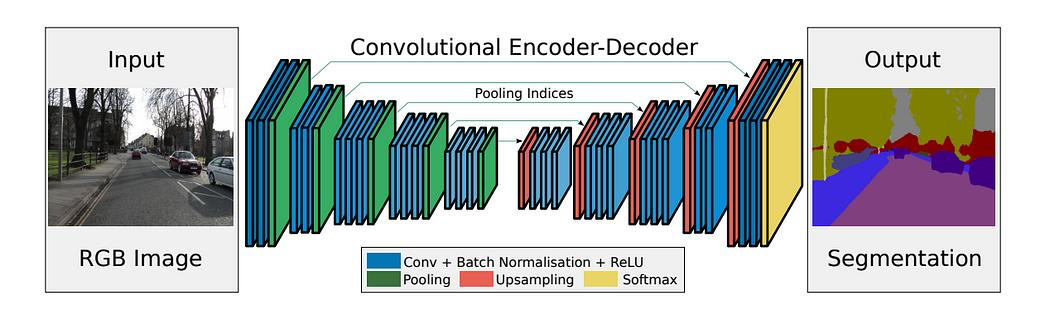
\includegraphics[width=450pt]{assets/segnet}
    \caption{SegNet Architecture Diagram}
    \label{fig:using:segnetarchi}
\end{figure}

\section{Implementation Trials 7/3/2024}
A pre-trained SegNet model [6] was tried to get setup in order to get to know the model implementations with SegNet. Here is a step-by-step process followed and the challenges faced along the way.

The Implementation was derived from an existing implementation found on the web.
% More details about the link....

First, the following libraries and packages were imported to the Google Colab environment.
\begin{lstlisting}
Cv2
Numpy
Pandas
Pickle
Tensorflow
\end{lstlisting}

After that dataset needed to be categorized as below to feed the dataset to the model without errors.
\begin{lstlisting}
data_path = 'Dataset/'

train_path = "Dataset/train/"
train_label_path = "Dataset/trainannot/"

valid_path = "Dataset/val/"
valid_label_path = "Dataset/valannot/"

test_path = "Dataset/test/"
test label. _path = "Dataset/testannot/"
\end{lstlisting}

During compilation, an error was found stating an indexing issue in Matplolib’s GridSpec to arrange a grid of subplot for visualizing image data.
\begin{lstlisting}
IndexError: index 0 is out of bounds for axis 0 with size 0
\end{lstlisting}

The error was fixed by having the random index generator to generate values starting from q1 instead of 0.

% TODO: What happened at implementing the default segnet model with the default dataset?

During the transition to a Roboflow dataset (more details in dataset chapter) the implementation of SegNet model by the subgroup was incompatible with the dataset generated by Roboflow and another obstacle was faced.

% \section{Key Takeaways}
% Implementing the SegNet model imposed several challenges due to the breaking changes in libraries and our lack of expertise in fixing some deeply rooted issues that required a more clear understanding of the libraries and the structure of the model.

% As the literature review of SegNet progressed, there were also explorations for other viable alternatives for SegNet by our team. During that process another better model called ENet was found and with the advice of the Supervisor, the project transitioned to testing ENet. This is discussed in more detail in the following chapters.

% Even though the current focus of the subgroup is ENet, a decision to keep reviewing the SegNet model and implementing it sometime was made to get more familiarity with the segmentation models.